\documentclass[dvipdfmx]{jreport}
% \usepackage{graphicx}
\usepackage[dvipdfmx]{graphicx}
\usepackage{sty/masterthesis}
%\usepackage{showkeys}%推敲用
\usepackage{lscape}	%横
\usepackage{mathptmx} % Timesへ
\usepackage{comment}
%\usepackage{booktabs}  %表結合
%\usepackage{multirow}  %表結合
%\usepackage{sty/slashbox}   %斜線
\usepackage{dcolumn}
\usepackage{array}
\usepackage{here}
\usepackage{enumerate}
\pagestyle{plain}
\makeatletter
\def\@cite#1{$\m@th^{\hbox{\@ove@rcfont #1)}}$} 
\def\@biblabel#1{[#1]}                              %参考文献[]へ
\def\@cite#1{{\mbox{\scriptsize{[#1}]}}}            %参考文献[]を文右へ
\makeatother
\setcounter{tocdepth}{2}                            % サブセクションも目次に出力
\begin{document}

% %----------------------------------------------------------------------
% % 表紙(年度,邦文題目,英文題目,指導教員,氏名,学籍番号を記入)
% % ※題目には適宜改行(\\)を手動で入れる
% %----------------------------------------------------------------------
% \年度{2023}
% \邦文題目{歯科インプラント治療における拡張現実を用いたサージカルガイドの開発と評価}
% \英文題目{Development and its evaluation of a Surgical Guide Using Augmented Reality for Dental Implantation}
% \指導教員{小林 茂, 桑久保 亮太, 平林 真実}
% \氏名{山岸 奏大}
% \学籍番号{22117}
% \表紙出力

%----------------------------------------------------------------------
% 目次
%----------------------------------------------------------------------
\contents

% 付図・付表のリストを作成する
\appendixpage{1}

%---------------------------------------------------------------------
% 1章 序論
%----------------------------------------------------------------------
\chapter{序論}
% 1.1 はじめに
%--------------------------------------------------------1.1 はじめに
\section{はじめに}
こんにち、一般に「直感的」で「使いやすい」ことは良いことであるされる。人々を取り巻く道具やインターフェースは、「人間中心設計」に基づき、「直感的」で「使いやすい」ものが目指される。人間中心設計とは、「システムの使い方」を人間工学やユーザビリティの知識と技術を用いて、より使いやすいシステムに最適化するアプローチである。「ユーザエクスペリエンスを向上させる」というときも、「使いやすさ」を目指すことが「向上」とされる。また、インターフェース研究者の渡邊は、自著「融けるデザイン」において、技術が個人の能力を拡張する上で、直感的に制御できるインターフェースの重要性を説いている。

確かに「使いやすさ」「直感的であること」が重要な場合もあるが、そうした経験のみが一辺倒に良しとされるべきではない。「使いやすさを設計する」ことは、予め定められた用途に行為を最適化することであり、これは人の行為や目的意識を限定するものだからである。

与えられた条件の中で自らのやり方を模索し「試行錯誤」する経験も重要であると考える。例えばピアノでは、奏者は手の大きさによる制約を受け、最初のうちは左右別々に指を動かすだけでも困難さを経験するが、ピアノの形を変えることはしない。試行錯誤を経て自分に合ったやり方で演奏できるようになったときの喜び、そして演奏中に独自のニュアンスを発見し、それが洗練されることで新たな奏法が生まれると考えられる。また、ミュージシャンのスキャットマン・ジョン(ジョン・ポール・ラーキン)は、「吃音症」という発話障害を持ちながらも、自身の身体をコントロールできないその症状を逆手に取り、「テクノスキャット」という独自の歌唱法を開拓した。「吃音」という障害と向き合いながら、単に歌唱法を発明しただけでなく、個人の存在のしかたを創造したと言える。

これらの例から、「試行錯誤」は人間にとって最小化されるべき無機質な経験ではないと考えられる。最初から使いやすく便利なものには、主体性を発揮する余地が少ない。試行錯誤から個人がやり方を見出すことで、高度なことが自在にできるようになる。またそれが、簡単に乗り越えられる経験ではないからこそ、乗り越えることに喜びもある。そして、道具や体験の設計に対しては、設計する人が想定する目的や範囲を超えた創発が個人から起こる可能性がある。したがって、ある目的に適合するよう最適化するだけでなく、試行錯誤を経験する余地を残すアプローチも重要であると言えるだろう。

\section{本研究の目的}
\section{本論文の構成}
\newpage

%----------------------------------------------------------------------
% 2章 関連研究
%----------------------------------------------------------------------
\chapter{関連研究}
\label{related_works}

本研究は、「身体化(embodiment)」の過程における、主観的な体験に着目した研究である。

「身体化(embodiment)」は心理学や認知科学の領域で、Botvinick \& Cohen(1998)によるラバーハンド錯覚の報告を皮切りに「身体化感覚(sense of embodiment)」を中心として実証的知見が蓄積されている。本章ではまず、「身体化感覚」の概要と、他分野での応用や発展について、具体的な研究を紹介する。

\section{身体化感覚(sense of embodiment)}

身体化感覚は一般に、身体に対する所有感(sense of body ownership)、行為主体感(sense of agency)、そして自己位置感覚(sense of self-location)を合わせた感覚として取り扱われる\cite{kilteni2012}。その元となったのは、Gallagherの「ミニマルセルフ」という概念である。「ミニマルセルフ」とは、自我としてみなしうる必要最小限のもののことであり、身体所有感(sense of ownership)、行為主体感(sense of agency)の二つから構成されていると説明される\cite{Gallagher2000}。

こうした自己についての説明を実験的に操作・検証可能としたのがBotvinick
\& Cohenによるラバーハンド錯覚\cite{BotvinickCohen1998}である。これは、自分の手を衝立の裏に隠し、偽物の手を目の前に置いた状態で、両方に同じタイミングで刺激を提示すると、偽物の手を自分の手であるように感じる錯覚である。この報告により、外界の対象への身体所有感の生起が可能であることが示されたとともに、身体所有感研究に関する系統的な手法が開発されることとなった。

そしてこの知見は、VR、ロボティクス、インターフェースデザインなどの領域での応用や、更なる基盤技術の開発へと発展している。

\section{VRにおける身体化感覚}

近藤ら\cite{Kondo2020}は、右手の親指の動きにVR上の左腕の動きを連動させることで錯覚的な身体所有感(Illusory Ownership)が生じるのかについて検証した。被験者は、右手の親指の動きがVR上での左腕の動きにマッピングされている様子をヘッドマウントディスプレイを介して確認する。実験では、被験者に5分間自由に指先を動かしてもらった後、VR上で左腕のあたりにナイフが突然出現する。このときの皮膚電導反応(Skin Conductance Response, SCR)の計測と、身体化感覚(embodiment)に関するアンケートを20人の被験者に行った結果、この手法を通して右手の親指と左腕の結びつき(re-association)は、程度は弱いが誘発できると報告している。

また佐々木ら\cite{sasaki2022multisoma}は、VR上で最大4つの身体を制御できるシステムを実装し、複数の身体を制御する際、人間の身体認知がいかに更新されるかについて検討した。実験では3つのタスクを設定し、視線情報、タスクのパフォーマンス、身体化感覚(sense of embodiment)についての主観評価により、これらの身体の認知を評価した。結果、人間は複数の身体を同時に操作することで、それぞれの身体に対して身体所有感(sense of ownership)や運動主体感(sense of agency)を持つことができると報告している。

\section{ロボティクスにおける身体化感覚}

Kielibaら\cite{kieliba2021robotic}は、ロボットで拡張された親指が人間の運動能力を拡張させることができるかどうか、そしてそれが手の神経表現や機能にどのような影響を与えるのかを調査するため、The Third Thumbというロボットの親指を用いた研究を行った。この親指は、足のつま先で操作することができる。
5人の参加者は、5日間にわたってThe Third Thumbを装着し、実験室での使用と日常生活での使用が求められた。通常は両手を使って行うタスクをこの親指を駆使して片手で行い、その器用さ(dexterity)や身体化感覚(sense of embodiment)などの度合いが評価された。トレーニングを経て、認知的負荷が増加した場合や視覚が遮断された場合でも、親指の運動制御、器用さ、そしてThe Third Thumbに対する身体化感覚(sense of embodiment)が向上したと報告している。

\section{インターフェースデザインにおける身体化感覚}
インターフェース研究者の渡邊は、ユーザインターフェースにおける「透明性」を実現する上で「自己帰属感(sense of ownership)」に着目した\cite{Watanabe2017}。
ここで「透明性」とは、道具の使用において、使っている最中にはその道具自体を意識せずに身体の一部になったかのようになり、目的に集中できるようにすることとされている。

そして、道具の透明性は「自己帰属感」によってもたらされると考え、マウスカーソルを対象に、ユーザインターフェースにおける自己帰属感を検証する「ダミーカーソル実験」を行った\cite{Watanabe2013}。この実験ではスクリーン上に、マウスと連動して動く通常のカーソ
ルの他に色形状の同じの複数のダミーのカーソルをランダムに動くように同時に提示する。被験者は動きのみでしか自身のカーソルを判別することができない環境になる。そしてこの実験によって、人は動きのみであっても複数のダミーカーソルの中から自身のカーソルを発見できると報告されている。どれが自分のカーソルか判別できることから、人間はカーソルに対しても自己を見出しており、自己帰属感が生起していると主張している。
これを踏まえて、ユーザインターフェースにおける自己帰属感を生起するために、操作時の動作とグラフィックの追従性が重要となることを指摘した。

\section{本研究の位置付け}

ここで紹介したVR分野やロボティクス分野での研究は、身体化の可能性や限界を探る研究であった。特に、VR分野での身体化研究は、身体全体の大きさや数など、扱える操作変数が多いため、新しい心理学研究の可能性を拓いていると言える。

インターフェースデザインにおける応用は、一般に身体拡張と呼ばれるような領域ではない人と道具の関係についても身体性の枠組みから捉える事例として、この枠組みの応用可能性を拡張していると言える。

しかしその一方で、本研究が着目するような、身体化するまでの過程における主観的な体験に関する研究が不足している。

ここで「身体化の過程」に注目すると、結果としては同じ身体化であっても、そこには質的な違いが存在することがわかる。例えばラバーハンド錯覚とThe Third Thumbは、いずれも身体化感覚が生起している点では共通する。しかし、前者は受動的な触覚提示によっても身体化が生じているのに対し、後者の身体化は「器用さ(dexterity)」を途中で獲得することで身体化が生じる。その過程では「もどかしさ」や「楽しさ」を経験すると考えられる。つまり、身体化するまでの意識的な試行期間の有無という点において異なっている。

% アバターに対して様々な介入が可能なVR分野では、身体拡張における可能性や限界を探る上で格好のフィールドであると言え、佐々木らや近藤らによる研究は、身体化感覚を評価軸とした様々な身体操作を実現するための基盤技術の研究であると位置付けられる。

% 一方Kielibaら\cite{kieliba2021robotic}の研究は、拡張された身体部位との協調(human-hand cooporation)が芽生えるまでの5日間という比較的長い調査期間を設け、身体化感覚の変化に着目している点で特徴的である。

そのため本研究は、身体化の過程での経験をより細かく説明するために、一般に用いられる「身体化感覚(sense of embodiment)」ではなく、コンピュータ工学研究者のSydney Felsによる身体化の程度についての分類を援用する。Felsは、人が対象に対してどのような感情を抱いているかに注目することで、「身体化」の程度を捉えた。これにより、身体化に関する新たな方向性を捉えることができるのではないかと考えた。

% \section{身体化感覚(sense of embodiment)との相違}
% 「Embodiment」という言葉は心理学研究やHCI分野において、一般には身体化感覚(sense of embodiment)を言及する意味において使用される。これは、身体に対する所有感(sense of body ownership)、行為主体感(sense of agency)、そして自己位置感覚(sense of self-location)を合わせた感覚として取り扱うことが多い\cite{kilteni2012}。
% この概念は「人間がいかに現実を認識しているか」を理解することで技術を発展させてきたバーチャル・リアリティ(VR)分野において実験的に操作・検証可能とするために整理されたものであるが、その元となったのは、Gallagherの「ミニマルセルフ」という概念である。

% 「ミニマルセルフ」とは、一切の自己知識を失ったとしても残る最小限の自己であり、身体所有感(sense of ownership, body ownership)、行為主体感(sense of agency)の二つによって支えられていると説明される\cite{Gallagher2000}。

% こうしたGallagherの説明を起点にそれらを評価する方法が考案され、ラバーハンド錯覚実験などにみられるように、生来の肉体ではないものを自分の身体と錯覚してしまうような人間の身体像の曖昧さに注目した研究が認知科学や心理学の領域で取り組まれてきた\cite{braun2018senses}。こうした研究で蓄積された実証的知見は、インターフェースデザインや身体拡張の設計・評価へと応用されている。渡邊がマウスカーソルやスマートフォンの道具としての透明性を説明する上で用いた「自己帰属感」も、Gallagherの「sense of ownership」に対する訳語である\cite{Watanabe2017}。

% しかし、この意味でのembodimentは、「人間の一部として対象が帰属しているような状態」についてのみ言及するものである。embodimentは日本語で「身体化、一体化、身体性」などと訳されるが、動詞の「embody」についてCambridge Dictionaryで引くと、
% \begin{quote}
%   \begin{enumerate}
%     \item \textit{to represent a quality or an idea exactly} (質や考えを的確に表すこと) 
%     \item \textit{to include as part of something} ((何かを)何かの一部として取り込むこと)
%   \end{enumerate}
% \end{quote}
% とある\cite{embody}。ここで指摘したいのは、2つ目の意味からembodimentの原義とは「何かを取り込んで、何かの一部とすること」であり、「人間の一部として対象が帰属しているような状態」のみを指すわけではないということだ。

% \section{身体の変換や拡張の試み}
% 身体の変換や拡張といったテーマは、embodimentの理論を踏まえて近年様々な研究が行われている。
% % 高度化・複雑化する技術が高い表現力や能力を持っていたとしても、それを扱う人間の能力が追いつかない限り、有効活用することができない。この問題は、群ロボット制御のような人間の身体性を越えた技術、そして身体の変換や拡張に取り組む分野で顕著に現れる。

% % Kimらは、複数台の卓上ロボット群を効果的に制御するための、インタラクション様式のセットと、そのデザインガイドラインを提示した。複数台で連携を取り合いながら、柔軟に役割を変えて複雑なタスクを達成することのできる群ロボットには、個々のロボットが持つ能力の総和以上の可能性がある一方で、それらを効果的に操作するためのインタラクション様式の設計に関する研究は少ない。そこで、卓上ロボット群に達成してほしいタスクを伝えられた被験者が、実際に卓上ロボットを前にしたとき、どのような働きかけをしてそれらを動かそうとするのかを観察することで、自然なユーザの動きを引き出すという手法(Elicitation Study)によって、様々なシチュエーションに対する適当なインタラクション様式を示した。

% % 稲見らによる自在化身体プロジェクト\cite{jizai}では、人間がロボットや人工知能などと「人機一体」となり、自己主体感を保持したまま自在に行動することを支援する「自在化技術」の開発と、「自在化身体」がもたらす認知心理および神経機構の解析をテーマにウェアラブル技術やバーチャル環境における共有身体の操作における基盤技術の開発に取り組む。
% 近藤らは、右手の親指の動きにVR上の左腕の動きを連動させることで錯覚的な身体所有感(Illusory Ownership)が生じるのかについての検証を、20人の被験者を対象に行なった\cite{Kondo2020}。モーショントラッキングを用いて取得された右手の親指の動きがVR上での左腕の動きにマッピングされている様子を、被験者はヘッドマウントディスプレイを介して確認する。実験では、5分間自由に指先を動かしてもらった後、VR上で左腕のあたりにナイフが突然出現する。このときの皮膚電導反応(Skin Conductance Response, SCR)の計測と、一体化(embodiment)に関するアンケートの結果から、この手法で錯覚的な身体所有感は確実に誘発できるものの、その程度は弱いと報告している。

% また佐々木らは、VR上で最大4つの身体を制御できるシステムを実装し、複数の身体を制御する際、人間の身体認知がいかに更新されるかについて検討した。実験では3つのタスクを設定し、視線情報、タスクのパフォーマンス、主観評価により、これらの身体の認知を評価した。結果、人間は複数の身体を同時に操作することで、それぞれの身体に対して身体所有感(sense of ownership)や運動主体感(sense of agency)を持つことができることがわかった。\cite{sasaki2022multisoma}。

% これらの研究は、親指の動きで動く左肩や複数の身体など、自分の肉体とは異なる身体ではあるが、それを自分の身体であるかのように認知しやすいものとそうでないものとの境界を探っていくこと、ひいては人間の認知的特性の理解に関心があると捉えられる。

% 一方で、次に紹介するKielibaらの研究は、同じく身体性(embodiment)についての評価が含まれるが、変換された身体のもとで行動する期間が長く、時間を経て身体性が獲得されることについて取り組んでいる。

% % 身体の変換や拡張を行う研究は近年、数多く行われている\footnote{近年に多いとする根拠は、小鷹の「ラバーハンド錯覚の遅い発見問題」という問題意識に基づく。小鷹は、「ラバーハンド錯覚」というシンプルな錯覚が学術的にはじめて発表されたのが1998年と遅く、それが「コンピュータの普及により、事物を情報的に処理する感受性が世界に浸透しつつあった1990年代後半」であったことに、単なる偶然ではない「情報としての身体」という発想を後押しするものがあったのではないかと指摘する\cite{kodaka}。}\cite{Kondo2020, ekusute,Kasahara2017,augmented_hand_series}。そうした実践の中心的な関心について、ここでは「錯覚」と「身体に対する再注目」であるとして、先行事例を紹介する。その上で、それぞれの関心と本研究の関心の相違点を説明することで、研究の位置付けを明らかにする。

% % しかし本研究の関心は「錯覚」ではない。そうではなく、突然自分の体とは似ても似つかない、それでいて扱い方もわからないような身体を与えられたときに、どう一体化していくかということに関心がある。

% % 小川らによる「えくす手(Metamorphosis Hand)」\cite{ekusute}では、指の伸びた手などの現実の身体にはあり得ない特性を持ったバーチャルな身体を通じてピアノを演奏することができる。そのねらいは、「現実とは異なる特性のバーチャルハンドへの身体所有感の生起を通じ、現実の身体的制約を超えたインタラクションを実現する、一種のバーチャルな身体拡張体験を提供する」と説明される。

% Kielibaら\cite{kieliba2021robotic}は、ロボットで拡張された親指が人間の運動能力を拡張させることができるかどうか、そしてそれが手の神経表現や機能にどのような影響を与えるのかを調査するため、The Third Thumbというロボットの親指を用いた研究を行った。この親指は、足のつま先を用いて操作することができる。
% 5人の参加者には、5日間にわたってThe Third Thumbを装着した状態で通常は両手を使って行うタスクを、この親指を駆使して片手で行い、その器用さ(dexterity)や身体性(sense of embodiment)などの度合いが評価された。トレーニングを経て、認知的負荷が増加した場合や視覚が遮断された場合でも、親指の運動制御、器用さ、そしてThe Third Thumbとの協調性が向上した。

% Kielibaらの研究では、体験者は身体が変換された状態を比較的長い期間経験し、参加者が特殊な能力を獲得していくことについての時間的変化を扱っている。これは近藤らや佐々木らの研究とは違い、身体の拡張の試みの中でも、人間の能力の獲得に関心があると捉えられる。こうした人間の能力の獲得の過程には、FelsのいうBelongingの意味での一体感(embodiment)が見られる。

% 本研究が身体の変換表現に取り組む理由は、後者のKielibaらの研究に見られる関心と共通している。つまり人間が自分の身体とは程遠い変換に対して、どのようにその扱い方を見出していくのかに関心がある。そのため本研究の中で探求する身体の変換表現においては、生来的に備わっている認知的特性によって一体感を得るのではなく、人間が意識的に注意を向けて体験することで一体感を得ることが重要である。

% ただし、本研究において取り組む変換の表現は、Kielibaらほど一体感を経験するまで長い期間を要するものではない。だが、短い期間であるからこそ人間が注意を向けている間の経験について、詳細に記述することが可能である。これらを踏まえると本研究の貢献とは、次章で説明する\textit{grasp}の概念を用いて、Intimacyが生じるまでの過程についての詳細な説明を可能にすることである。

% 身体所有感の生起要因に関するこれまでの議論を参照し、本作は「テクスチャ、形状、空間的配置、解剖学的構造の4つの特性」を根拠に、身体所有感が生じながらも、自己身体と意味的に類似しないバーチャルハンドを制作している。これらの特性は、身体所有感を生じさせる上での実証的知見ではあるが、本研究が対象とするIntimacyは、例えば楽器のように、こうした生起要因を押さえなくとも、習得を経て生じうるのではないかと考える。また、生起要因を多く踏襲しているわけではないからこそ、身体所有感が生じるまでには期間を必要とし、その程度にも個人差が生じるのではないだろうか。これらの観点から、本研究の取り組みは「えくす手」よりも極端な身体変容を促す体験として位置付けられる。

% \subsection{身体に対する再注目}
% Golan Levinらによる《Augmented Hand Series》\cite{augmented_hand_series}は、ウェブカメラによって取得した体験者の手の映像をリアルタイムに変形し、指の本数や長さなどの異なる手を投影する作品である。また、佐藤雅彦らによる「君の身体を変換してみよ展」では、さまざまなアプローチで身体の変容を扱う作品が展示されたが、その中でも《点にんげん・線にんげん》\cite{sato_icc}という作品では、動物の関節などの位置を示す点の動きだけでも脳が「生物的な動き」としてひとまとめに認識できる(バイオロジカルモーション)という現象を活用し、体験者の関節の位置が表示された点群が、様々な方法で結びつけられたり、ある役割を与えられるなどの「変換」に対して、「自分の身体である」という認識が保たれたまま形が変わっていく作品である。

% これらの作品の関心は、「身体に対する再注目」であると考えた。いずれも、身体が異なる見た目に変わったというだけであって、実用的な特別な能力が付与されたり、ゲーム性があるわけではない。それでも身体を動かしてみることの動機は、「動くこと」そのものへの興味が働いているからである。これは、生後まもない乳児が自分の手の存在に気づき、手を見つめたり、動かしたりしながらよく観察する動作である「ハンドリガード」に似た現象であると解釈した。「身体の変換」を通して、新しい身体像を得たことから生じた「注目」と向き合う契機となる。

% こうした関心の作品を、ここでは生まれ持った肉体に対する「注目」を最初と数えて、「身体に対する再注目」とした。


\newpage

%----------------------------------------------------------------------
% 3章 システム開発/分析手法
%----------------------------------------------------------------------
\chapter{\textit{Grasp}モデルについて}
\section{モデルの概要}
「grasp」は「把握」を意味する動詞・名詞だが、日本語でも物体を把持する手の動作であると同時に、概念について理解するときにも用いる。ここでの\textit{grasp}とは、「人がある対象に注意や目的意識を抱き、注意を向けた対象を確かめるため、または目的の達成に向けて試行を行う期間」のことを指す。手指の構造を変化させる本作は、このコンセプトに注目し、手指の変換をきっかけに起こる注意や、変換した手指とボールとの関係のもとで生じる目的意識が、体験者の中で自発的に生まれることを目指した。
本研究では、作品体験についてのインタビューを通してそれが実現していたことを示し、そのデザインプロセスと最終的な作品形態についての考察を通して、\textit{grasp}の設計に向けた指針となることを目指す。
\section{既往研究との比較}
\subsection{Felsによるインタラクティブ・アート評価の4つのカゴリー}
\textbf{Response}: a case where the person perceives the object to be separate from their own self. 

\textbf{Control}: the person feels like the object is an extension of their self. Fels describes this intimate
relation as occurring quite quickly within Iamascope due to the system’s prompt visual feedback [8].

\textbf{Contemplation}: not an interactive one. In this relationship the person sees their self as separate from the object. this relation as similar to that between a painting and its viewer.

\textbf{Belonging}: the person feels like the object is controlling them and they get pleasure from being thus controlled.
\newpage

%----------------------------------------------------------------------
% 4章 実験結果 
%----------------------------------------------------------------------
\chapter{修士作品 Grasp(er)}
\section{概要}
ここまで、身体性の変容をその契機として「技量の問題による使いにくさ」を経験することについてFelsの分類に基づいて整理を行い、前の\ref{graspについて}章で\textit{grasp}の定義を行った。

本章では、そうしたコンセプトに辿り着くまでに行ったプロトタイピングについて整理すると共に、作品の概要を述べる。さらに、前章に示した概念を体現するものとして制作した修士作品《Grasp(er)》においては、この概念がどのように適用されているのかについて説明する。\\

\section{制作プロセス}
本節では、最終的な作品形態に至るまでのプロトタイピングについてと、その過程で構築されたライブラリの開発について説明する。
\subsection{プロトタイピング}
本作品の形態に至るまでに、総計60パターンのプロトタイプ制作を行なった。プロトタイピングにおける目的を時系列で3段階に大別すると、「コンセプトメイキング」、「変換表現によって錯覚する「手触り」についての発散」、そして「変換表現で異なる身体動作が引き出される要素の特定」である。「コンセプトメイキング」に至るまでのプロトタイピングについては、前章にて説明した。ここでは、後の2つについて説明する。

\subsubsection{変換表現によって錯覚する「手触り」についての発散}
変換された手指を見ながら自分の身体を動かしていると、独特の気持ちよさや、ある動きをしようと力が入る感覚がある。物理的に何かに触れているわけではないが、何もないところで同じ動きをしていても知覚することのない、視覚情報と手指の運動の対応関係によって生じる身体感覚を、ここでは「手触り」と呼ぶ。
プロトタイピングの中で、変換表現の形状、マッピングの方法、推定された手指の姿勢情報の時間操作などを通して、この「手触り」にどのような幅が存在するのかについて探った。
\subsubsection*{形状}
形状については、指を動きの最小単位として、指ごとに独立したバリエーション、指同士を直列に繋ぎ合わせたバージョン、円形に繋ぎ合わせたバージョンなどを作成した。また、単位である指をどのように表現するかについては、「円形」、「くの字」、「ひょうたん型」などのバリエーションで表現を試みた。
\begin{figure}[H]
  \centering
  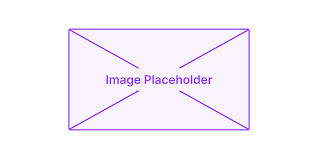
\includegraphics[width=15cm]{img/placeholder.png}
  \caption{ユニットのバリエーション}
  \label{fig:unit_valiation}
\end{figure}
\subsubsection*{マッピングの方法}
マッピングについては、1つの動きを複製して、1つの動きを複数のパーツの動きへと波及させるバリエーションなどを作成した。図\ref{fig:networked_finger}に示すプロトタイプでは、指先をクリックすると5本ある指のうちのいずれかの動きを追従する指が、指先に追加されるものである。どの指が付け加わるかはランダムで、指が新しく追加されるたびに、それがどの指の運動であるかを同定するには、一本一本指を動かして、どこがその指に対応しているのかについて同定する必要がある。
\begin{figure}[H]
  \centering
  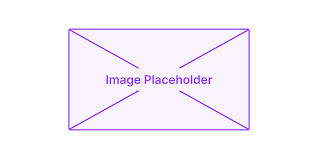
\includegraphics[width=15cm]{img/placeholder.png}
  \caption{Networked Finger}
  \label{fig:networked_finger}
\end{figure}
\subsubsection*{手指の姿勢情報の時間操作}
最新の自分の動きだけを表示するのではなく、過去の動きも表示するプロトタイプにも取り組んだ。図\ref{fig:prototype_delay}に示すプロトタイプでは、5本の指の動きが等間隔に並べられているが、それぞれの指は、鉛直上向きの角度に現在の指の動き、そこから時計回りに、順次過去の指の動きが並べられている。このプロトタイプでは、指先を小さく動かすと、その動きが時計回りに伝播していくようすが見て取れる。これは例えばゼリー状の物体を触れた時のような、衝撃が物体全体へと伝播していくようすに見立てられるため、柔らかいオブジェクトに触れているときのような身体感覚を錯覚することがある。

\begin{figure}[H]
  \centering
  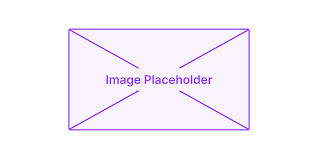
\includegraphics[width=15cm]{img/placeholder.png}
  \caption{過去の動きを用いた例}
  \label{fig:prototype_delay}
\end{figure}
\subsubsection{変換表現でIntimacyが引き出される表現への収束}
ここまで行なってきたプロトタイプから、以下の2つの観点から方向性を絞り、ブラッシュアップを試みた。
\subsubsection*{制御している感覚が強く引き出される表現}
1つ目の観点として、手指の微細かつ複雑な動きをもって、緻密な制御をしているという感覚が引き出される表現へと絞り込んでいくことにした。\\
その上で注目したのは、「関節を折り曲げる動き」に対する共感性である。\\
人間の手指は
その一方で、円の半径に関節の動きをマッピングさせるような表現については、縮んだり、膨らんだりする動きには共感しづらい。微細な運動が増幅される「気持ちよさ」があるが、この気持ちよさは身体動作との連動によってもたらされる気持ちよさではなく、動作に対するフィードバックに対する快、すなわちFelsのいう「Response」による快が強い。経験されるため採用しなかった。\\
さらに、1つの動きを複製して円形に配置したり、フラクタル的に配置するパターンを排除した。これについては、グラフィックデザイナーの女性が体験した際「構造としては緻密であるのに、動きは単純であるように感じる」と意見した。その理由として彼女は、「対称性が前面に出ているため、シンボルとしての印象を強く感じてしまう」「意識していないところも同時に動いている感覚があるため、自分の動きだと思えない」からではないかと推測した。

\subsection{ライブラリの開発}
本作品を構成するにあたり、基本的な関数をまとめたライブラリを開発した。ライブラリには、円滑に体験するための補完処理を実装している。
具体的には、ガウシアンフィルターによる平滑化処理、トラッキングが途切れた際の例外処理の2つである。

\subsubsection*{ガウシアンフィルターによる平滑化処理}
推定精度の問題から、モデルより推定される姿勢情報をそのまま出力すると、手指を動かしていなくても小刻みに振動したり、一時的なフレームレートの低下に起因してスムーズに動作していないように感じることがある。\\
そこで、体験者にフィードバックする際に使用する姿勢情報は、前後2フレーム分のフレーム情報にガウシアンフィルターを適用した平滑化処理を実装している。ただし、トラッキングが開始した直後は5フレーム分のフレーム情報を使用することができないため、この場合は取得できる限りのフレーム情報を用いて同じ処理を行なっている。そのため以下では、各フレーム情報に対する重みづけと、それを用いて体験者に提示される姿勢情報を求める上での一般式を示す。
モデルより推定された最新の姿勢情報を\(P_{n}\)、出力されている姿勢情報を\(S\)とすると、
  % 平滑化フレーム S の定義
  \begin{equation}
    S = \sum_{i=-2}^{2} w_i' \cdot P_{n+i}
    \end{equation}

ここで、\(w_i'\)は正規化されたガウシアンフィルタの重みを表す。正規化前の重み\(w_i\)は、
\begin{equation}
  w_i = \frac{1}{\sqrt{2\pi}\sigma} e^{-\frac{i^2}{2\sigma^2}}
  \end{equation}

正規化された重み\(w_i'\)は、
  % 重みの正規化
  \begin{equation}
  w_i' = \frac{w_i}{\sum_{j=-2}^{2} w_j}
  \end{equation}
と表現される。
この処理のため、最良時で60fps程度で取得される姿勢情報は、慢性的に0.3sほどの遅延を伴って体験者にフィードバックされることになる。

\subsubsection*{トラッキングが途切れた際の例外処理}
体験時、環境光や、手指を動かす範囲や速度の関係から、トラッキングが途切れることがある。素早い動きをしている最中に1フレームでも途切れると円滑に体験することができないため、この時は例外的に、トラッキングが途切れる直前のフレーム情報で失われたフレーム情報を埋め合わせる処理を実装した。また、トラッキングが途切れていることに起因する不快感は、本作品の体験外の問題なので、手指の動きがトラッキングできていない状態を視覚的にフィードバックするため、トラッキング不能時に塗りつぶしを透過する視覚効果を実装した(\ref{fig:opacity})。

\begin{figure}[H]
  \centering
  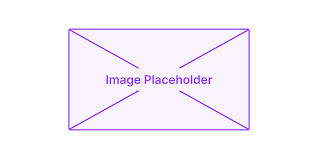
\includegraphics[width=15cm]{img/placeholder.png}
  \caption{トラッキング不能時の視覚効果}
  \label{fig:opacity}
\end{figure}

\section{作品構成}
一方で、プロトタイピングを通して同定した変換表現を通して生じた異なる身体像に対する共感覚のようなものは、変換された手を用いた作業に移行した瞬間に、注意が向きづらくなるといった課題が起こった。そこで、最終的な作品としてはその2つを分けて構成した。

\subsection*{Familiar / Strange}
「Familiar / Strange」は、手指の配置や関節の数・位置が次々と変化していく作品で、手の運動に対する再注目が起きることを目指している。作品は最初、手の形がそのまま現れた状態から開始し、指の並びや関節の配置の変化が起きる。一本一本の指がくの字の形をして積み上げられる様子をピークに、逆順に変化が巻き戻され、再び元の手の形に戻るという、3分10秒で1ループの構造となっている。
\begin{figure}[H]
  \centering
  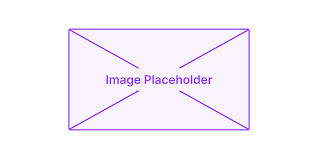
\includegraphics[width=15cm]{img/placeholder.png}
  \caption{Familiar / Strange}
  \label{fig:familiar_strange}
\end{figure}

\subsection*{Relation}
「Relation」は、変化した手指を取り巻く関係が次々と変化していく作品で、手と直接的に制御できないボールの関係性におけるGraspに焦点を当てている。1つ目の作品と同様、最初は手が表示された状態から始まり、段階的に並び替えられた手指を覆う皮膜が現れ、ボールが現れる。最後は的が現れ、的を取るたびにボールの大きさが小さくなり、3つ連続して取ると、皮膜は消え、再び元の手の形に戻る。
トラッキングされた手指の位置が、手首から指ごとに分割され、左端から右へ、左手の小指から親指、そして右手の親指から小指の順に整列される。しばらくすると、指先以外の運動が捨象され、残された指先を結ぶ線が現れる。ここで、現れた線によって再び全ての指が1つのまとまりとして統合されることになるが、その線は後に現れるボールに対して衝突判定が適用される、新しい構造の手指を覆う皮膜のような機能を有する。皮膜のある領域を外れるとボールは下方に落下するが、そのあとは再び画面の中央にボールが出現する。
さらに一定時間が経過すると、皮膜の上方に白い点が現れる。白い点に対してボールを当てると、ボールは一回り小さくなり、ボールを落とさずに合計3回白い球に当てると、ボールは消失し、皮膜が現れるときと逆の順序を辿って画面の中の手は再びもとの形状に戻る。
\begin{figure}[H]
  \centering
  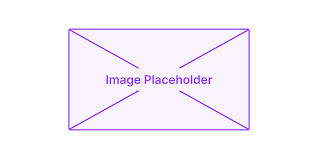
\includegraphics[width=15cm]{img/placeholder.png}
  \caption{Relation}
  \label{fig:relation}
\end{figure}

この作品は、1つめの「Familiar / Strange」と異なり、構造が変化した手指と、ボールという直接的に動かすことができない対象との関係性に注意が向けられることをねらいとした。

\section{修士作品に対する\textit{grasp}の適用}
\subsection{基本構造}
「身体の変容」を扱っている本作では、取得されたキーポイントの位置を大きく変更させることで、「意図的にIntimacyを下げる」操作を行なっている。しかし「下がった」という事実を体験者が認識するために、もとの手が鏡合わせのように出力されている状態から、徐々に形を変えていくようすを連続的に示すモーフィングを実装している。\\
過去に展示していたバージョンではモーフィングを示さず、手指が認識されたとたんに全く違う手指が提示される作品形態であった。しかし、この形態で展示した場合、画面の中の手指と自身の関係性について、全く異なる生命体のようなものを、操り人形のように自分の手指の指令によって動かす、といったような関係性として認識されることがあった。また、全く見慣れない形なので、「手指を細かく動かせる」といった、作品がもつ可能性に気づけない場合があることがわかった。そこで、このモーフィングを実装することで、白い点が関節を表していること、そして手指の運動を細かくトラッキングしていることを事前に伝え、それが形を変えた姿として画面の前に提示されていることを示す形態を採用することになった。
そうすることで、画面に出力されているグラフィックと身体との関係性は別々の存在ではなく、自分の身体であったことが明示される。\\
\subsection{Familiar / Strange}
この作品は、3分10秒で1ループの構造になっている。それぞれの変換は、線形補完やゴム紐が切れた時のような振動を伴う動きによって補完される。シーン遷移を説明する図を以下に示す。
\begin{figure}[H]
  \centering
  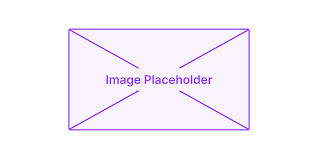
\includegraphics[width=15cm]{img/placeholder.png}
  \caption{Familiar / Strange}
  \label{fig:diagram_familiar_strange}
\end{figure}

\subsection{Relation}
\newpage

%----------------------------------------------------------------------
% 5章 結論
%----------------------------------------------------------------------
\chapter{バリデーション}
\section{実験概要}
\subsection{Video Cued-Recall メソッド}
インタラクティブ作品の評価方法にはさまざまな評価が存在するが、本作品を評価する上では、体験時、体験者がどのようなことに注意を向け、どのような行動を取ったかについて精緻に振り返る必要がある。そのため本研究では、体験者に体験時のようすをできるだけ詳細に表現してもらうため、Video Cued-Recallというメソッドを用いてデータの収集を行なった。 Video Cued-Recallとは、体験時のようすが記録された映像を視聴しながら、体験者本人が映像を手がかりに作品での体験を回顧し、言語化する方法である。インタビューを通して回顧するよりも詳細に体験を振り返ることができ、また体験しているそのときに体験のようすについて語ってもらう方法よりも、自然な体験について記述できることがその利点として挙げられる。

\subsection{参加者について}
インタビューは、FabCafe Nagoyaでの展示に際して、4名の体験者を対象に実施した。ただし、うち1名は「Relation」の体験時、トラッキングの精度が著しく低下していたため、1つ目に体験した「Familiar / Strange」の体験についてのみ調査の対象とした。

\subsection{データ収集}
参加者にはまず、調査の大まかな流れについて説明し、撮影についての許諾を得た。コンセプトの説明が自然な体験に影響することを避けるため、作品の体験の前にはコンセプトや具体的な作品の内容については説明せず、トラッキングされた手が次々に形を変えていくこと、手の形が表示された状態から始まり、再びもとの手の形に戻るループ構造のある作品であること、というインタビューに必要な最低限の構造のみ伝えた。

体験のようすは、手もとのハンドトラッキングを行うカメラ映像、現在時刻、体験者が実際に見ているスクリーンの映像が図\ref{fig:record_monitor}のようにレイアウトされて記録される。

\begin{figure}[H]
  \centering
  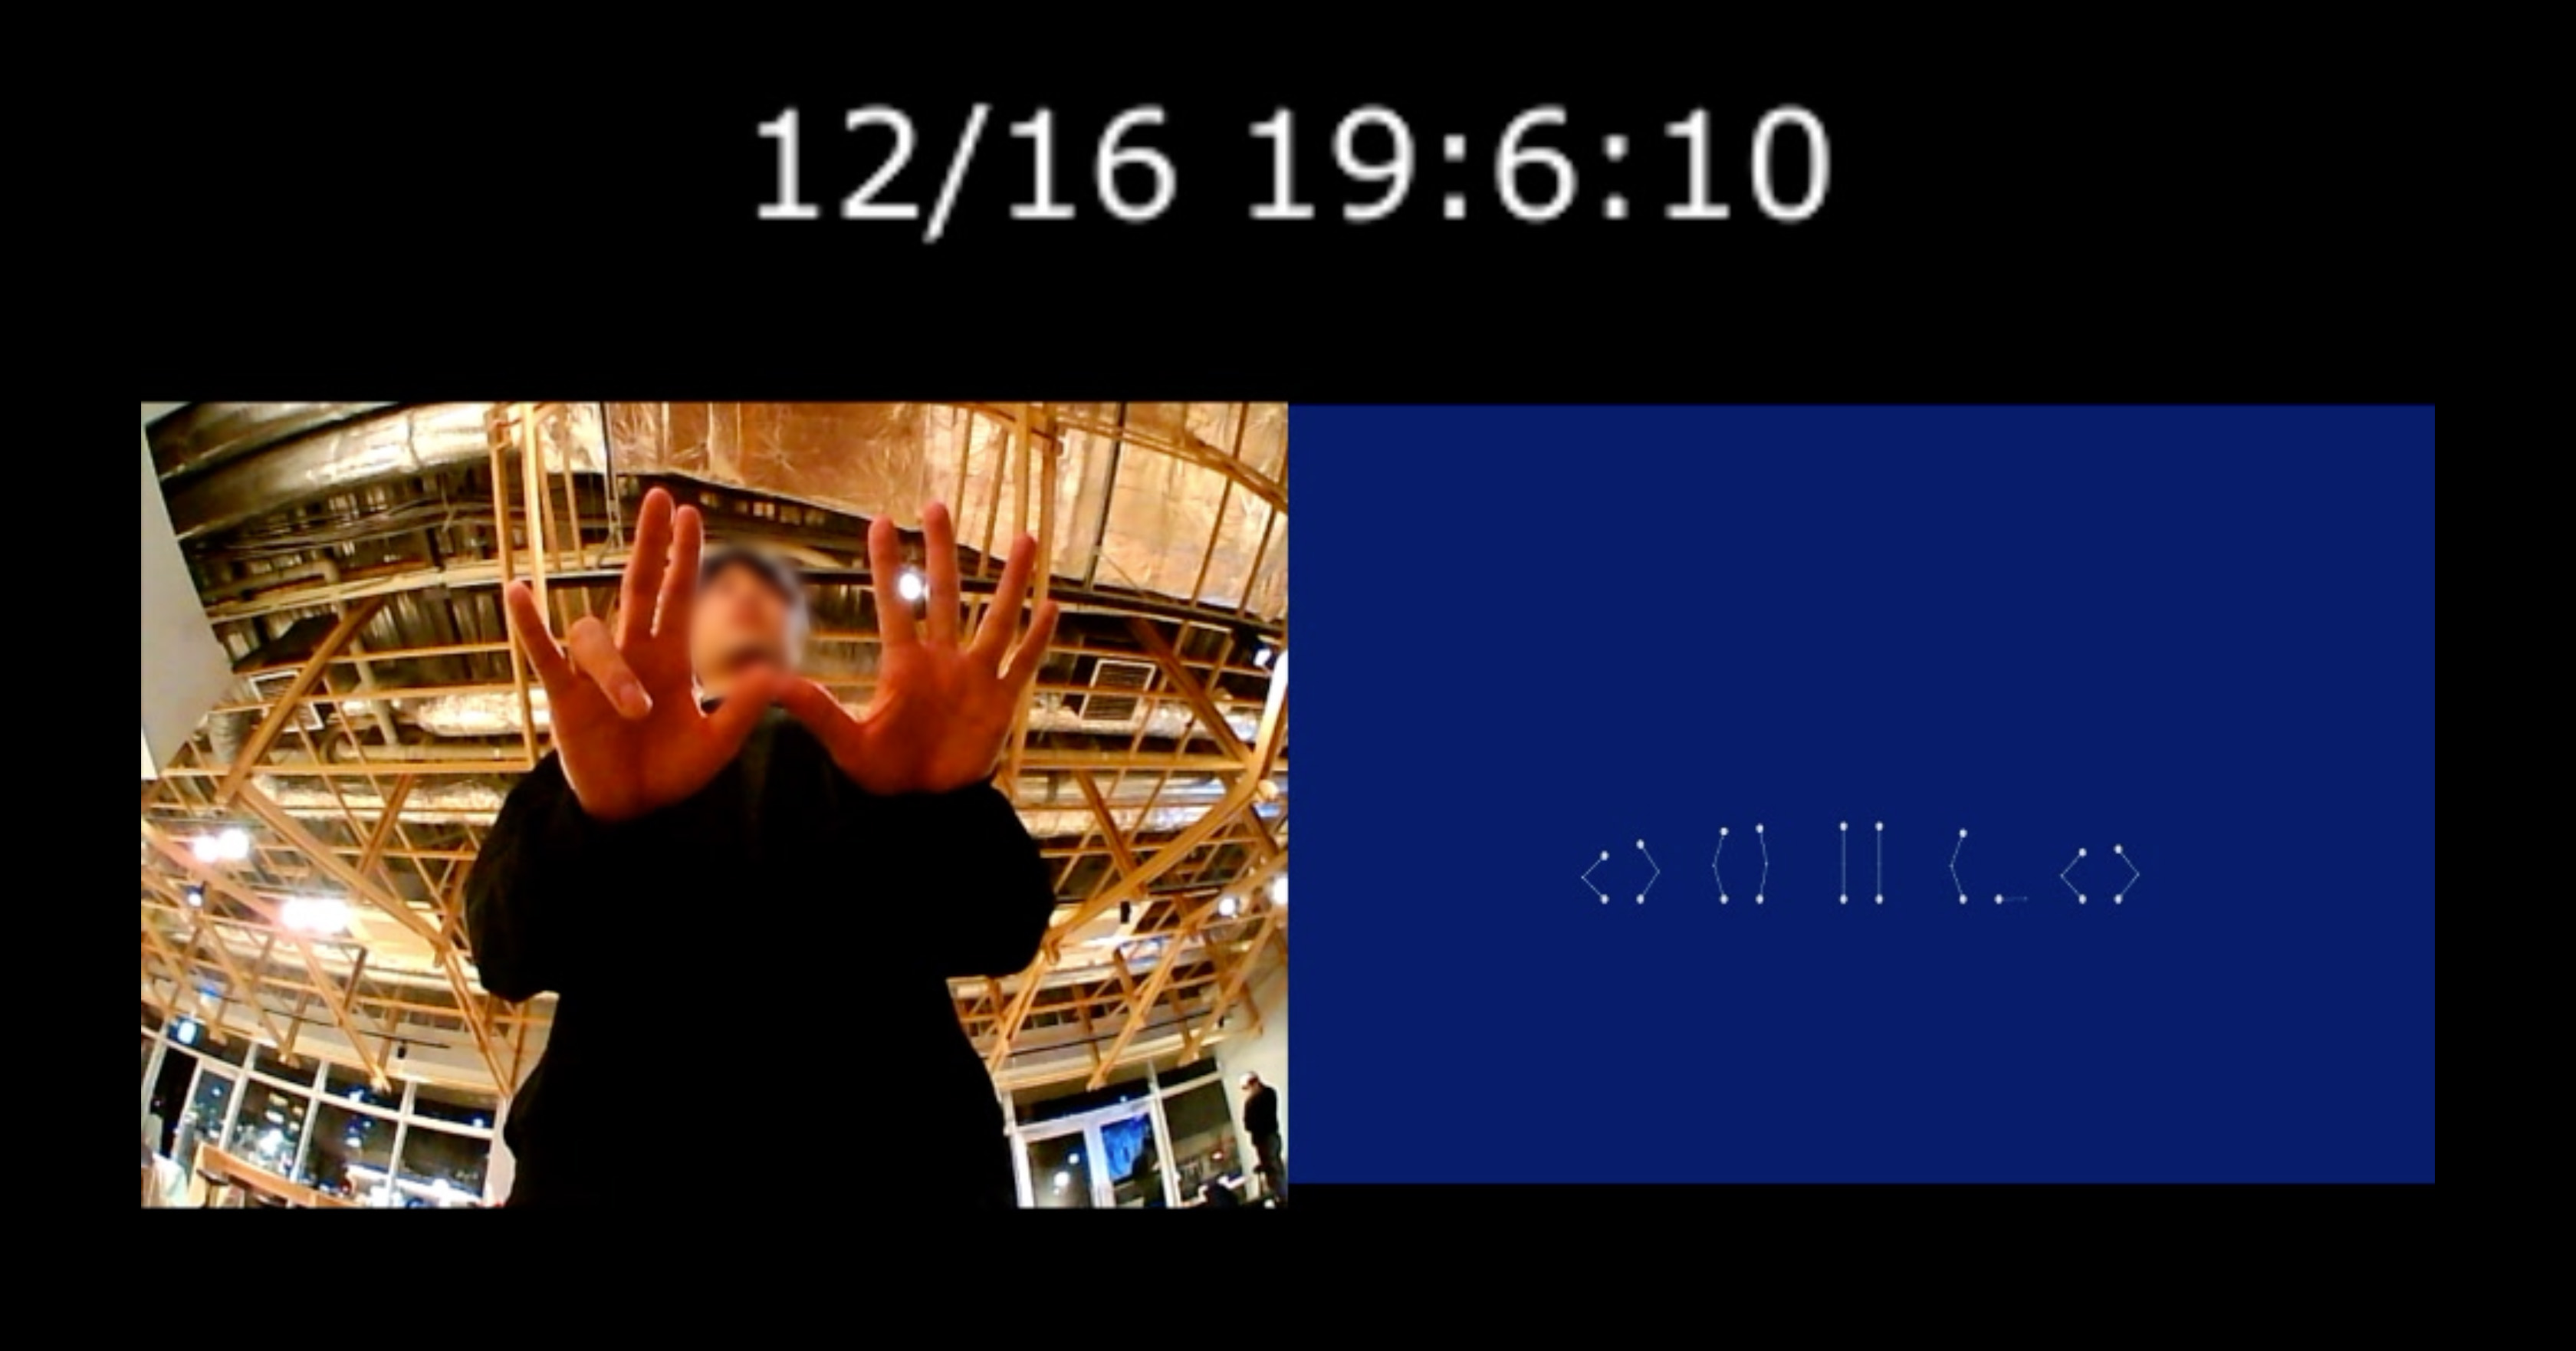
\includegraphics[width=15cm]{img/record_monitor.jpg}
  \caption{体験のようすの記録映像}
  \label{fig:record_monitor}
\end{figure}



\subsection{結果}

\newpage

%----------------------------------------------------------------------
% 5章 結論
%----------------------------------------------------------------------
\chapter{考察}
\label{考察}
本章では、\ref{validation}章で説明した結果を踏まえ、それぞれの作品において、どのような\textit{grasp}が芽生えていたのか、そしてそれを通して、参加者はこの作品をどのように受け止めていたのかについて考察する。

\section{Familiar / Strange}
参加者1と2では、挙動を確認するための動き、すなわちResponseの動作が見られた。

さらに、体験の中でプリミティブな図像であるためか、何かしらの「見立て」をしていることが多いとわかった。参加者1は、指が縦方向の動きのみに拘束されてパタパタと上下する形になったときに、ピアノの演奏のような身体感覚を想起していた。また参加者4は、「頭の中で既視感を作って」体験していたと振り返る。こうした「見立て」が生じることは、体験する人がそこに目的意識を見出して、対象を捉えようとすることの表れと考えられる。

何かしら参照できる他の身体動作や、見立てが可能であることが、体験の中で目的意識や注意を自分で作って体験することにつながるのではないかと語っている。
一方で参加者3は、手でフレームを作るような動きをしており、それに対して画面の中の手は思うように形ができず、「途中から飽きていた」と語っていた。
指一本一本の単位で手指の構造が切り替わっていく構成ではあったが、そうした画面の変化について「認知が追いつかなかった」と振り返り、手指を使って形を作っていたというイメージに対して、画面の中の振る舞いがそれとは全く異なることについて注意が向かなかったのではないかと考える。
また、「楽しみを探れた」という意見もあった。
\section{Relation}
興味深いのは、体験におけるもどかしさについてはトラッキングの精度とはあまり関係していないという点である。

参加者1は、。また参加者3は、
これは、初めて体験する人にとって、トラッキングが途切れていることがもどかしさとして経験されるほど、Intimacyは高まっていないということが示唆される。
参加者1は、

インタビューを通して得られた結果について、本作で試みていたコンセプトと照らし合わせた上で、達成できたこと、できなかったことについて考察する。

シビアな身体動作が求められるような目的意識と、そうでないものがあるということがわかった。「ボールを的に当てる」といった、明確な正解が存在する動きについては、指のトラッキング精度が低下していることに対して不快感を訴える意見があった一方で、「Familiar / Strange」ではトラッキングができていなくてももどかしいと感じるような意見は少なかった。
体験者1は、「気持ちよさを感じるポイントは、ゲームを進めていく中で変化してったけど、最初は「球を上げる」っていう目標になって、それを達成する気持ちよさを超えて、次の目標が見つかったときには、的に当てないと気持ちよくない」と振り返った。

さらに、「思い通りに動く」とは「連動性が担保されていること」ではないか、という仮説が新たに生じた。「思い通り」という言葉は、相手に命令する立場からすると、期待している結果と実際の挙動が一致している際に生じるが、「control」の状態下での「思い通り」とは、参加者4が体験を振り返るコメントにもあるように、「トラッキングができて」いて、「時差を極力なくし」た動きが「自分の思い通りの動きになってくれる状態」、すなわち「連動性」ではないかということが示唆された。その上で、「Belonging:帰属感」のようなIntimacyが生じるためには、その動きがさらに細かく制御できていることが重要ではないかと考えられる。

\section{今後の展望}
本節では、今回の研究では言及することができなかったが、今後このコンセプトをより発展させていくにあたり、論じていく必要があると考える2つの論点について整理する。1つは、青木淳による「原っぱと遊園地」、もうひとつは、ミゲル・シカールの遊び論について、ホイジンガとの比較から松永によって名付けられた「ふざけた遊び」に関する議論である。

\subsection{「原っぱと遊園地」}
楽器は、表現したいことが滞りなく表現できるようになるためには、習得も必要で、触れて直ちに使いこなせるわけではないという点において、「使いにくい」と説明することもできる。しかし楽器は結果として「使いにくい」わけだが、意図して「使いにくい」体験を設計している、というわけではないだろう。そうではなく、道具を通して達成されること(楽器であれば、演奏するという用途)、人間の身体的特性を考慮した上での最適化された合理的な形状であって、「使いやすさ」を目指すわけにはいかない部分が多いということだ。建築家の青木淳は、建築においてそこで行われることをあらかじめ決定されているような空間を「遊園地」とし、一方で行われることで空間が作られていくような空間を「原っぱ」と呼び、分類している。

\begin{quote}
  ともかく、廃校になった機能主義的小学校の空間は、ちょうど原っぱのように、人間にそれ に対するかかわり方の自由を与える。 原っぱとは、つまり空き地である。 宅地が造成され区画 される。これは人工的な営みである。 塀が築かれ、土地の形がきちんと確定される。一度は土地が均され雑草が刈り取られる。 そこまで行って、なにかの理由で、放置される。時間が経過して、 セイタカアワダチソウなどの雑草が、背丈ほど伸びてくる。そして、原っぱができ上がる。 更地というだけでは、原っぱではない。放置後の、適切な度合いの自然の遂行を必要とする。 
  廃校になった牛込原町小学校は、原っぱと同じく、人間の感覚とは一度は切れた決定ルールによって生成し、しかしその決定ルールが根拠を失った空間だったのである。そうして、偶然に、そこで人がつくることと、与えられる空間の規定力の対等が実現されていたのである。  
\end{quote}


楽器は、決定ルールが「使いやすさ」を設計する態度から自由であるという点において、「原っぱ的自然」を持つプロダクトであると言える。こうしたプロダクトに対して、メディアアーティストの久保田は「使いやすさ」を超越して「使いたさ」の重要性を説く。

\begin{quote}
  楽器は、リアルタイムに音を生成、コントロールするための道具である。そのインターフェイスの使いやすさが重要になるのはいうまでもない。 しかし、ピアノのインターフェイスは「はじめての人にも使えるように」あるいは「一目でわかるように」デザインされているだろうか?ギターは?トランペットやサックスの場合は?いずれの楽器も、 はじめての人にとっては音を出すだけでも四苦八苦の、使いにくい道具である。にもかかわらず、人はそんな使いにくい楽器に対して時間をかけてじっくりと向き合い、日々練習を重ね、少しずつスキルを向上させながら美しい調べを自在に奏でる夢を見る。そうした営みを支えているのは、人々の願いやビジョンである。(中略)「使いやすさ」のためにも、何よりもまず「使いたい」という願望が必要である。「どうやってやるか」ということよりも「何をやるか」のほうが先に来る。 豊富な機能を生かすも殺すもインターフェイス次第であることは間違いないが、その豊富な機能を使いたいと思えなければしょうがない。考えてみれば当然だ。 携帯電話のテンキーによる文字入力が良い例だ。何も工夫していないものが、結局は一番使いやすいインターフェイスになっている。重要なのは、表面的な改良ではなく、大きさや重さ、速度といった基本的な要目だ。妙な工夫をするよりもむしろ、シンプルであればあるほどスキルが活躍する余地が生まれる。ワンタッチで具体的なインターフェイスよりも、システマティックで抽象的なインターフェイスのほうが、多様な使用法とアウトプットを生み出すことができる。その名人芸と形容したくなるほどのスキルを生み出しているのは、人々の欲望だ。ここでも、欲望さえあれば、指が勝手に動いていく。技術革新の速度はそれなりに速いのかもしれないが、その気になった人間の適応力や柔軟性による変化の速度はもっと速い。人間の可能性は、底知れない。
\end{quote}

\subsection{シカールの「ふざけた遊び」}
こうした「原っぱ」的なプロダクトに対して、本研究が期待するような関わり方について述べるのは、ミゲル・シカールによる遊び論で語られる、「ふざけた遊び」の性質を持った遊び心の発露であろう。\\
遊びは存在のためのポータブルな道具である。ゲームに代表されるような遊びの「形式」よりも、「世界のうちに存在するモードの一種」としての遊び、つまり人間が人間としてあるあり方のひとつとしての遊びである。遊びは文脈に依存する。これは遊びが、物や環境やテクノロジーや人などからなる、その都度の「文脈」を使うかたちで生じるということだ。シカールの考えでは、もともと遊びのためにデザインされたものであるはずのゲームのルールですら、その本来の目的を無視して流用してしまうのが、遊び心という態度であり、遊びという「人間存在のモード」なのだ。\\
本研究が着目した\textit{grasp}のコンセプトは、こうした人間の感情の発露を期待する。その意味で、誰もが同じようにそれに価値を見出すような、一般的な利便性よりも、属人的な楽しさを志向したアプローチであると言えるだろう。
\newpage

%----------------------------------------------------------------------
% 5章 結論
%----------------------------------------------------------------------
\chapter{まとめ}
\newpage


%----------------------------------------------------------------------
% 謝辞
%----------------------------------------------------------------------
\chapter*{謝辞}
清々しい気持ちでこのページを書いているつもりが、書いてみてようやく自分の至らない点や、自分自身まだわかりきっていない部分が露呈して、実際には軽く吐き気がしています。しかしそれらを整理して再構成するには時間があまりに足りないので、論文執筆を通して指導いただいたことをもとに、時々思い返しては自分自身で赤入れをしていこうと思います。\\
主査の桑久保 亮太教授、副査の平林 真実教授には、度重なるアドバイスと作品・論文の審査をしていただきました。概念を曖昧にして用いていた点についての指摘を受けて論点を整理していく中で、いっそう明確になりました。\\
主指導教員の小林 茂教授には、研究内容にかかわるアドバイスに加え、論文執筆に際してはパラグラフごとのまとまりとパラグラフ間のつながりについて、細かく指導していただきました。応えることのできなかった指摘も多いとは思いますが、教わった作法は今後しっかりと身体化(embodiment)させていきたいと思います。\\
小林ゼミの小南菜子さん、太向弘明さん、成瀬陽太さん、そして聴講の松井美緒さんには、素朴な疑問から鋭い指摘まで、同じ学生同士だからこその忖度のない、貴重な意見をたくさんいただきました。私は今年で卒業ですが、この経験をみなさんの研究活動に還元していくことができたらと思います。また合宿にもいきましょう\footnote{それと、論文執筆に追われていたため未遂に終わった忘年会をやりたいです。}。\\
最後に、インタビューにご協力いただいた皆様、展示の機会を設けてくださったFab Cafe Nagoya様、IAMAS22期生の皆様、そのほか多くの研究にご協力いただいた皆様\footnote{列挙したらキリがなく、ひとまとめにしてすみません。これを執筆している今、お世話になった人々が、走馬灯のように頭の中を駆け回っています。あなたのことを、忘れていません。お会いしたときに直接感謝を伝えさせてください。}に深く感謝申し上げます。

\addcontentsline{toc}{chapter}{謝辞}
\newpage

%----------------------------------------------------------------------
% 参考文献
%----------------------------------------------------------------------
% \input{contents/references.tex}
\bibliographystyle{sty/sieicej}
\bibliography{references}

%----------------------------------------------------------------------
% 付録
%----------------------------------------------------------------------
\newpage
\appendix
\include{Appendix_model}

% \label{付録}
% \chapter{付録}


\end{document}